\documentclass[]{article}

\usepackage{amsmath}  % AMS math package
\usepackage{amssymb}  % AMS symbol package
\usepackage{bm}       % bold math
\usepackage{graphicx} % Include figure files
\usepackage{dcolumn}  % Align table columns on decimal point
\usepackage{caption}
\usepackage{subcaption}
\usepackage{hyperref}
%\usepackage{multirow} % Multirow/column tables

\begin{document}

\title{PHY 905 Project 1: Monte Carlo simulation of the 2D ferromagnetic Ising model}

\author{Steve Hughey}

\date{\today}

\maketitle

\begin{abstract}
A simple Fortran implementation of the Metropolis algorithm for Monte Carlo simulation of the Ising model of ferromagnetism is described. Results are presented for energy and magnetization over a range of temperature.
\end{abstract}

\section{\label{sec:intro}Introduction}

In statistical mechanics, the Ising model is a mathematical model of ferromagnetism in a $d$-dimensional lattice. 

\subsection{\label{sec:ising}Ising model}

The energy $H$ of the $N_x \times N_y$ lattice is a sum over all nearest neighbor spin products, multiplied by an interaction strength $J$:
\begin{align}
H =& -J \sum_{<i,j>} s_i s_j
\end{align}

The magnetization $M$ of the lattice in a given state is computed as a sum over all spins in the lattice:

\begin{align}
M =& \frac{1}{N_x N_y}\sum_{i} s_i
\end{align}

\section{\label{sec:imp}Implementation Details}

At each step of the Monte Carlo iteration, a lattice site $i$ is chosen at random. The spin $s_i$ of this site is negated with probability $e^{-\Delta E_i / k_B T}$. Boltzmann's constant $k_B$ is set equal to $1$ for convenience, so that the temperature $T$ is measured in units of $k_B$.

The change in energy $\Delta E_i$ due to negating the spin of a single point $i$ in the lattice is computed as the sum of $i$'s nearest neighbor spins multiplied by the new spin $s_i$ and the interaction strength $J$:

\begin{align}
\Delta E_i =& J s_i \sum_{<j>} s_j
\end{align}

\subsection{\label{sec:alg}Algorithm}

The Monte Carlo Ising model algorithm comprises the following steps:

\begin{enumerate}
 \item Choose a temperature $T$ and maximum iteration count $N_{iter}$
 \item Initialize lattice with all spins up
 \item Compute initial total energy $H$ and magnetization $M$
 \item Iterate $N_{iter}$ times:
 \begin{enumerate}
  \item Select a lattice site $i$ at random
  \item Compute the change in energy $\Delta E_i$ due to negating the spin at lattice site $i$
  \item If $\Delta E_i < 0$, retain the flipped spin value at site $i$, compute the change in magnetization, and update total energy and magnetization
  \item Otherwise ($\Delta E_i > 0$), retain the flipped spin value at site $i$ with probability $e^{-\Delta E_i / k_B T}$; if retained, update energy and magnetization
 \end{enumerate}
\end{enumerate}

\section{\label{sec:res}Results}

A Fortran code was written which implements the 2D Ising model. The source code can be found in the \href{https://github.com/hugheyst/ising}{GitHub repository}. The results in this section were obtained using a $(N_x,N_y) = 50 \times 50$ lattice with all spins up as the initial state. Plots with temperature on the horizontal axis were obtained by averaging the final 50,000 values of energy and magnetization from an iteration with $N_{iter} = 1 \times 10^6$.

\begin{figure}[ht!]
 \centering
 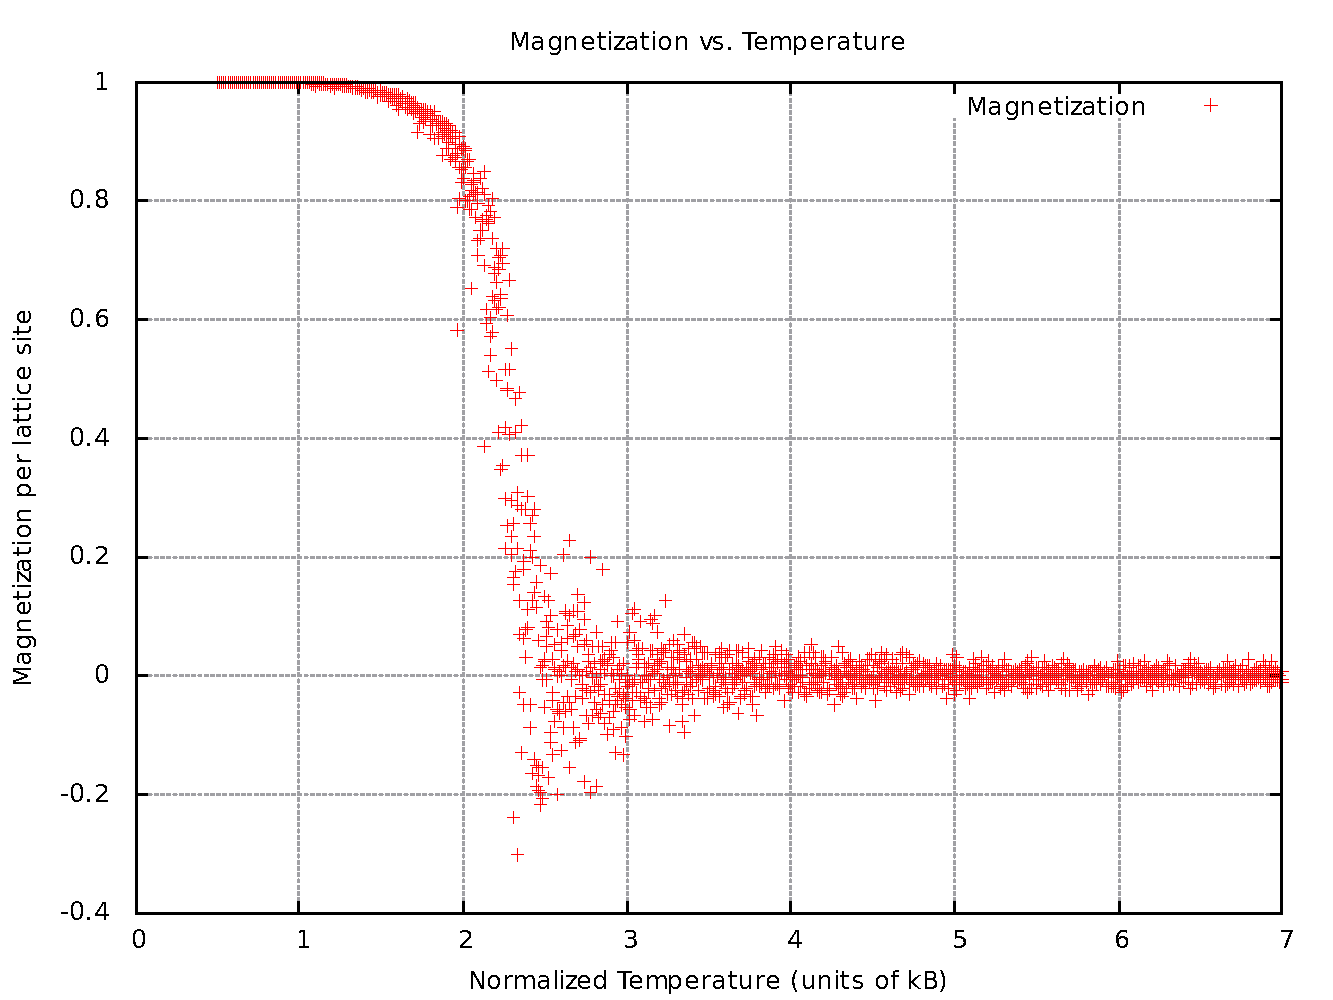
\includegraphics[width=\linewidth]{figures/mag_vs_temp.pdf}
 \label{fig:mag_vs_temp}
 \caption{Magnetization per lattice site from $T=0.5$ to $T=7$. Values computed by averaging final 50000 Monte Carlo iterations per temperature value.}
\end{figure}

\begin{figure}[ht!]
 \centering
 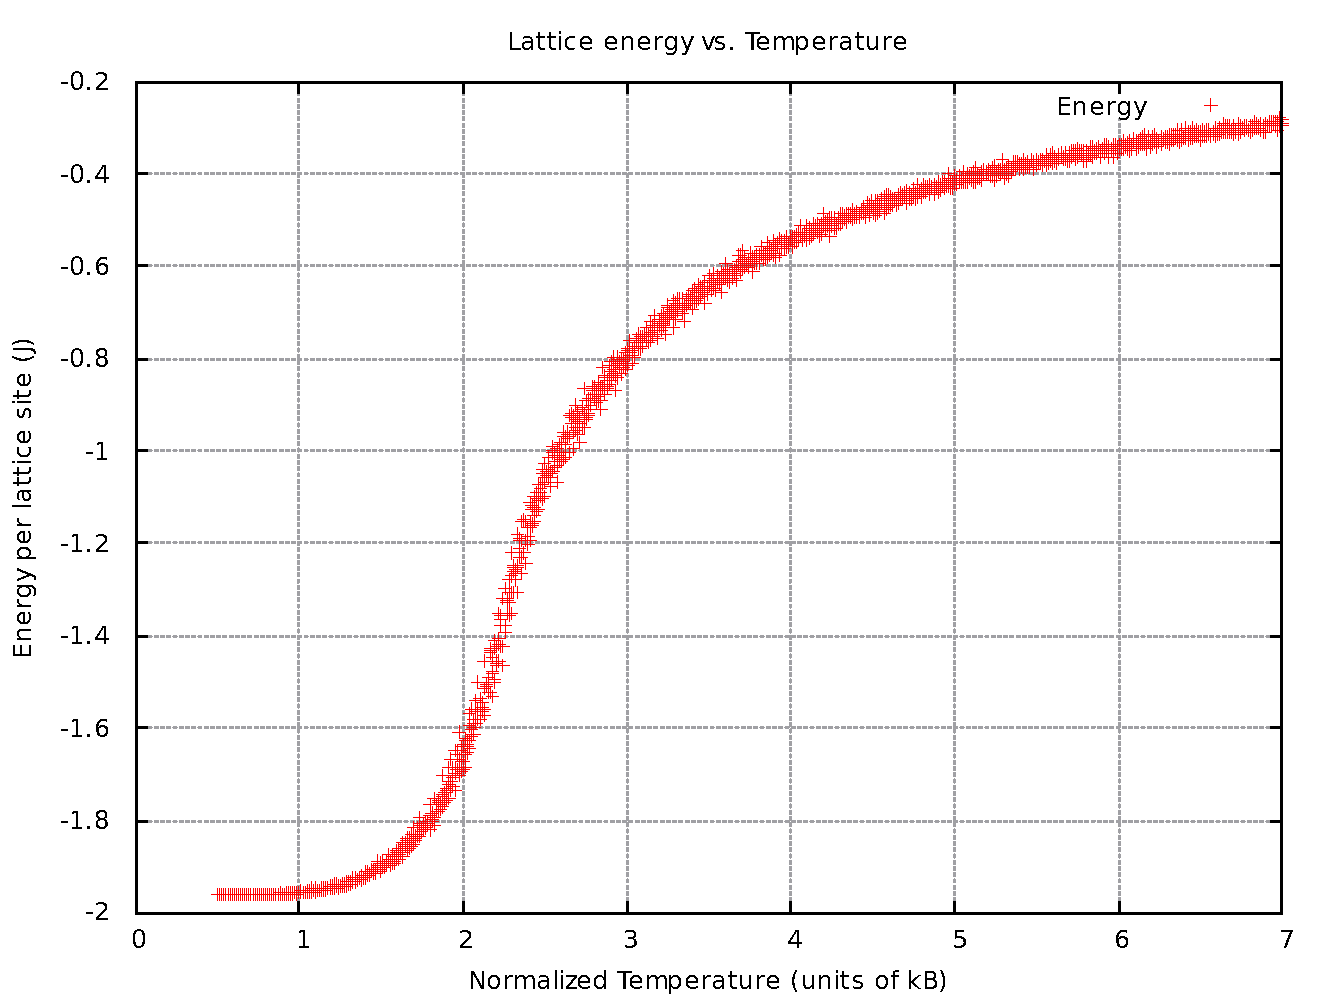
\includegraphics[width=\linewidth]{figures/energy_vs_temp.pdf}
 \label{fig:energy_vs_temp}
 \caption{Lattice energy per lattice site from $T=0.5$ to $T=7$. Values computed by averaging final 50000 Monte Carlo iterations per temperature value.}
\end{figure}

\begin{figure}[ht!]
 \centering
 \begin{subfigure}[b]{0.3\linewidth}
  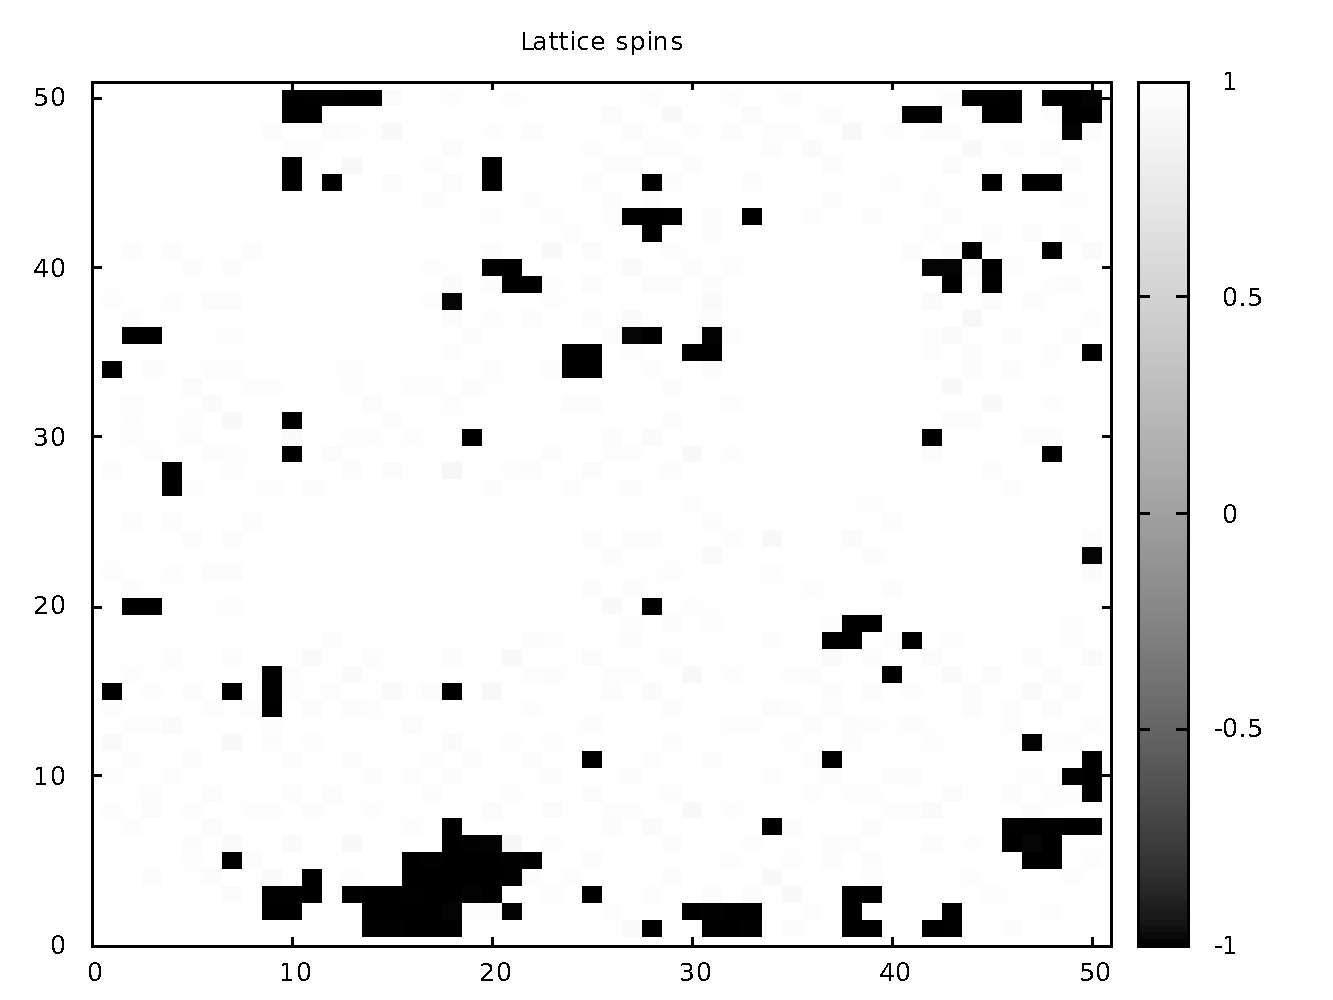
\includegraphics[width=\textwidth]{figures/spin_T_eq_2.pdf}
  \caption{$T=2$}
  \label{fig:spin_t_eq_2}
 \end{subfigure}
 \begin{subfigure}[b]{0.3\linewidth}
  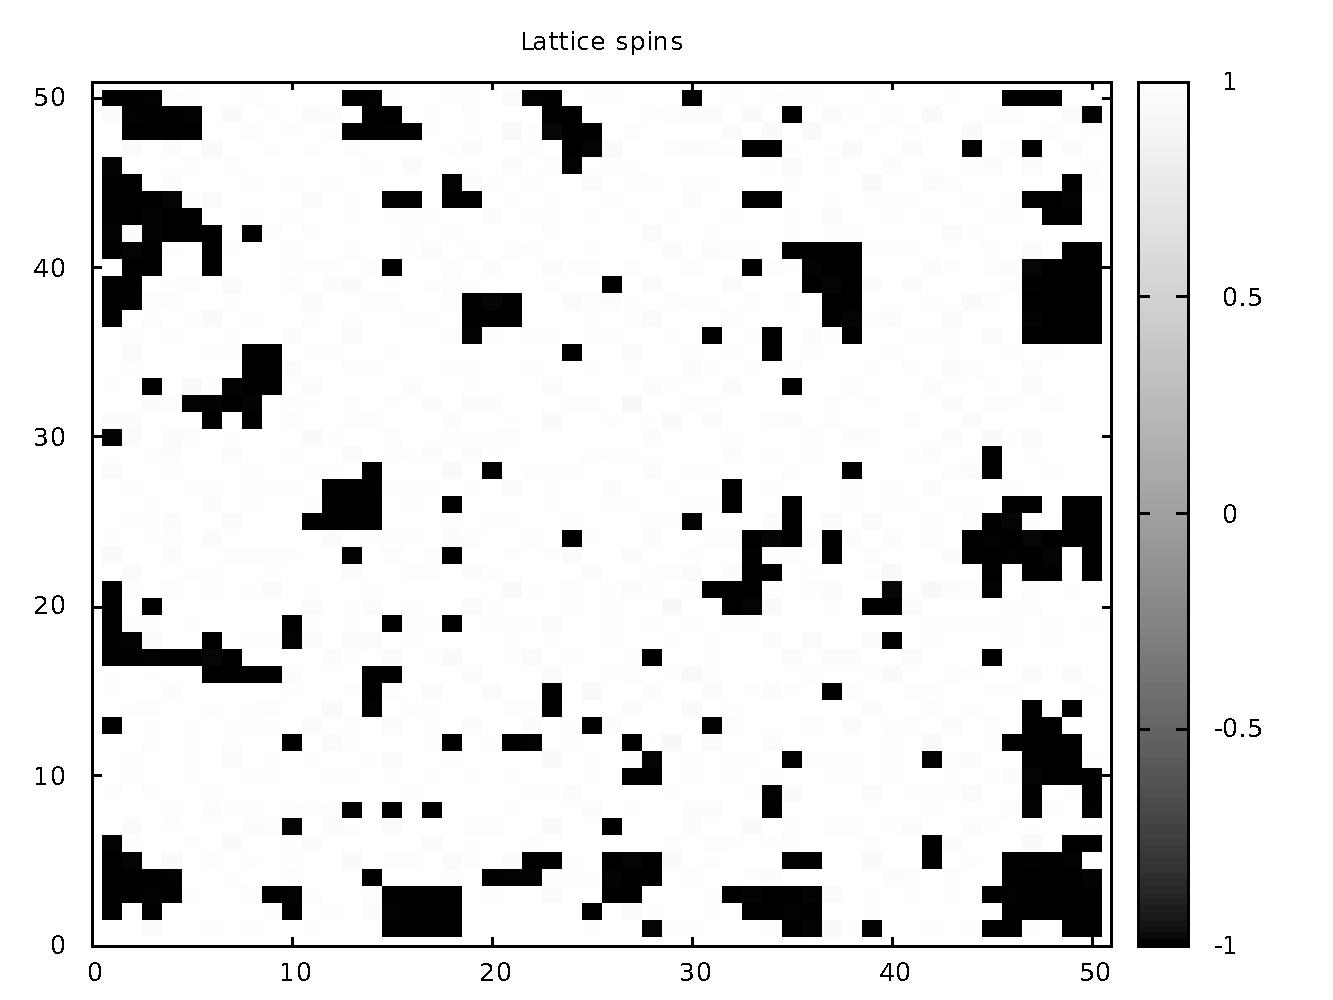
\includegraphics[width=\textwidth]{figures/spin_T_eq_2p2.pdf}
  \caption{$T=2.2$}
  \label{fig:spin_t_eq_2p2}
 \end{subfigure}
 \begin{subfigure}[b]{0.3\linewidth}
  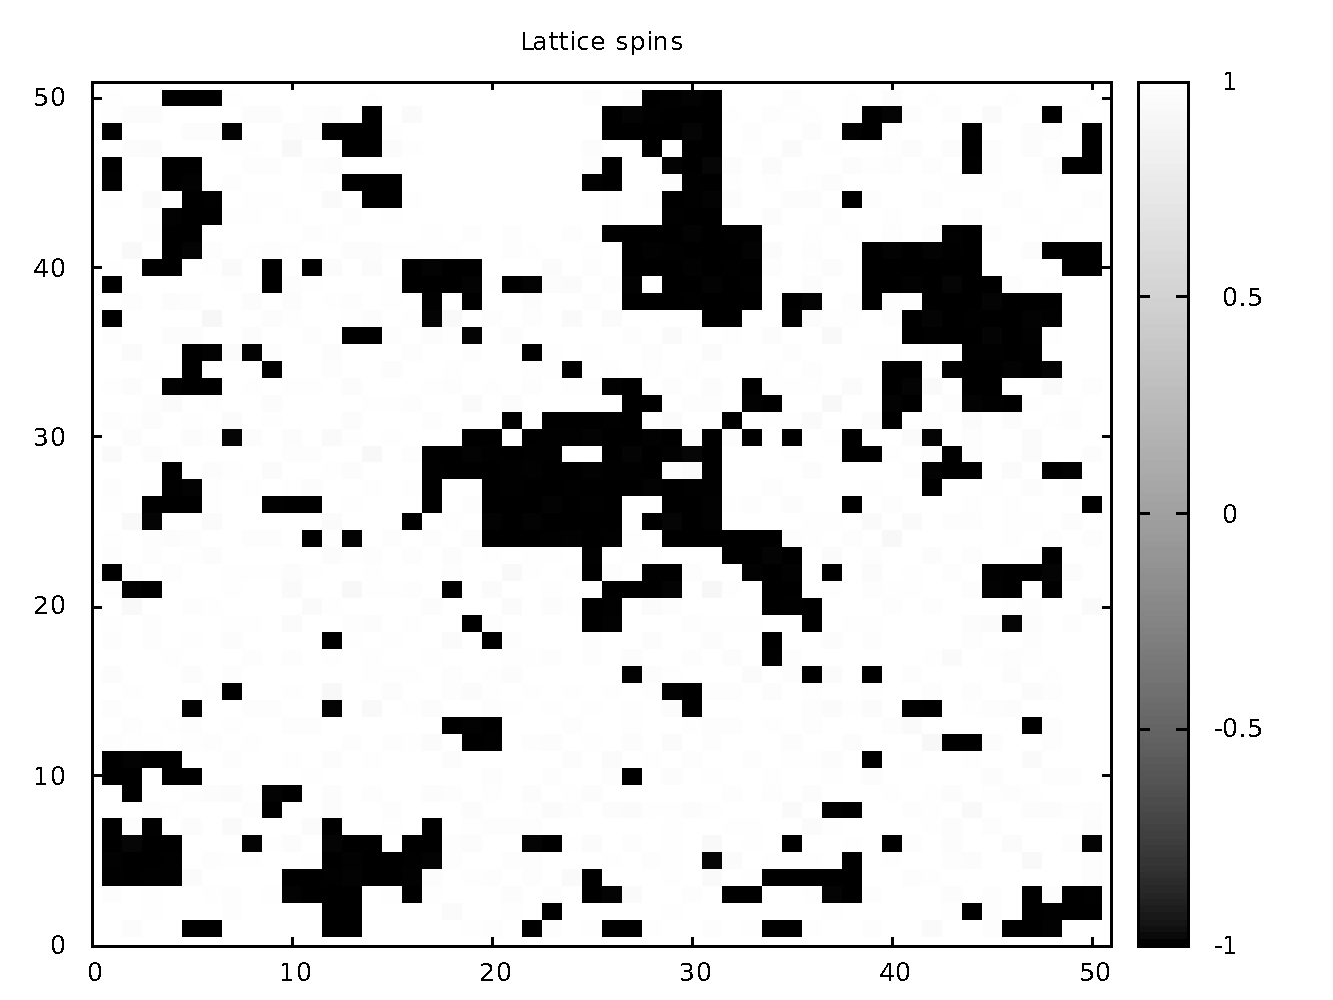
\includegraphics[width=\textwidth]{figures/spin_T_eq_2p25.pdf}
  \caption{$T=2.25$}
  \label{fig:spin_t_eq_2p25}
 \end{subfigure}
 
  \begin{subfigure}[b]{0.3\linewidth}
  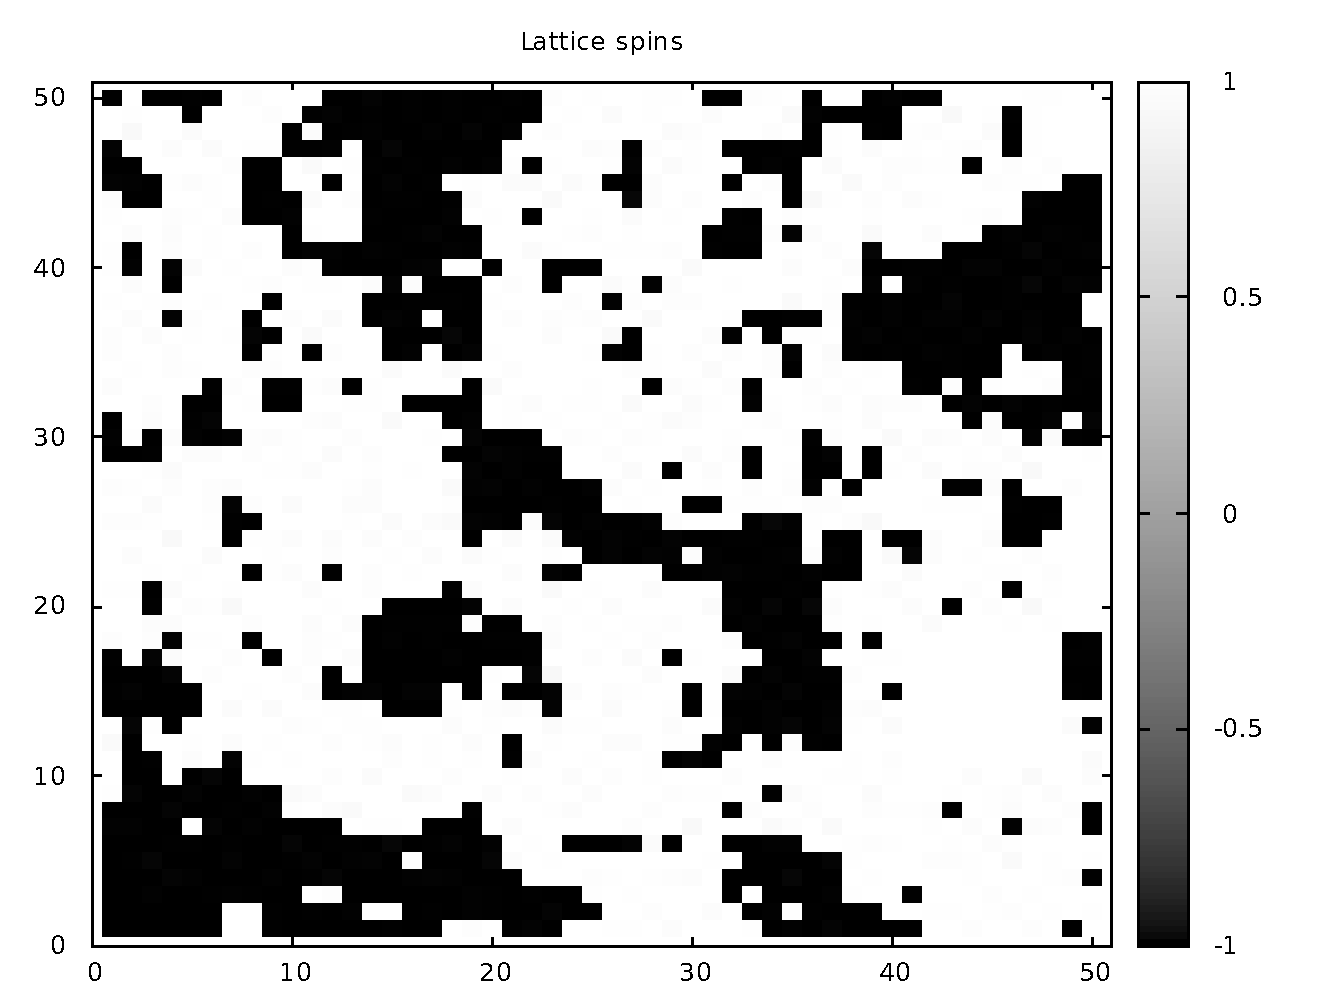
\includegraphics[width=\textwidth]{figures/spin_T_eq_2p3.pdf}
  \caption{$T=2.3$}
  \label{fig:spin_t_eq_2p3}
 \end{subfigure}
 \begin{subfigure}[b]{0.3\linewidth}
  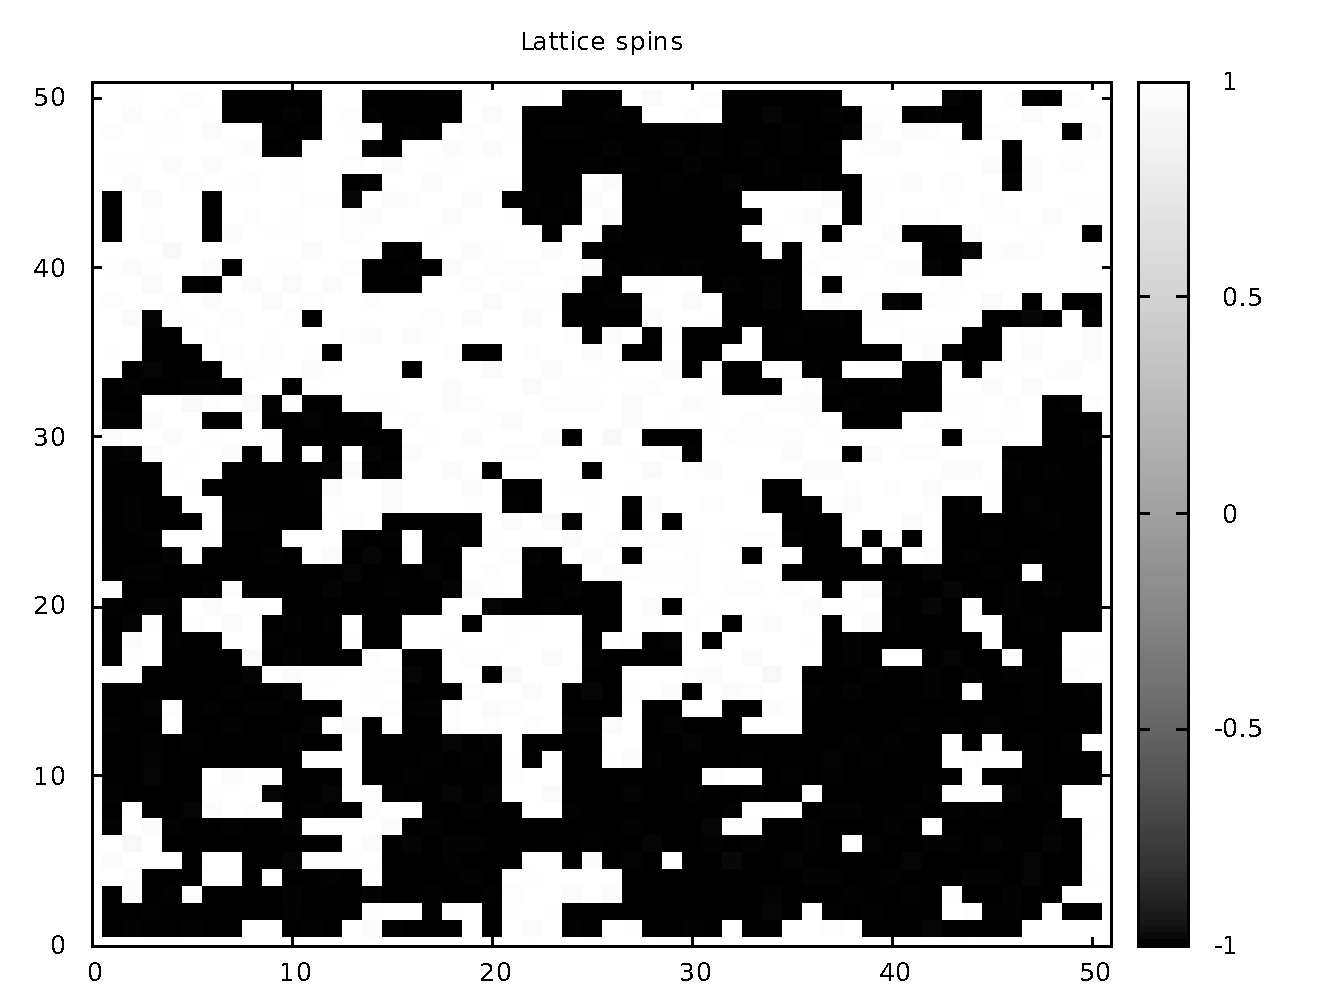
\includegraphics[width=\textwidth]{figures/spin_T_eq_2p5.pdf}
  \caption{$T=2.5$}
  \label{fig:spin_t_eq_2p5}
 \end{subfigure}
 \begin{subfigure}[b]{0.3\linewidth}
  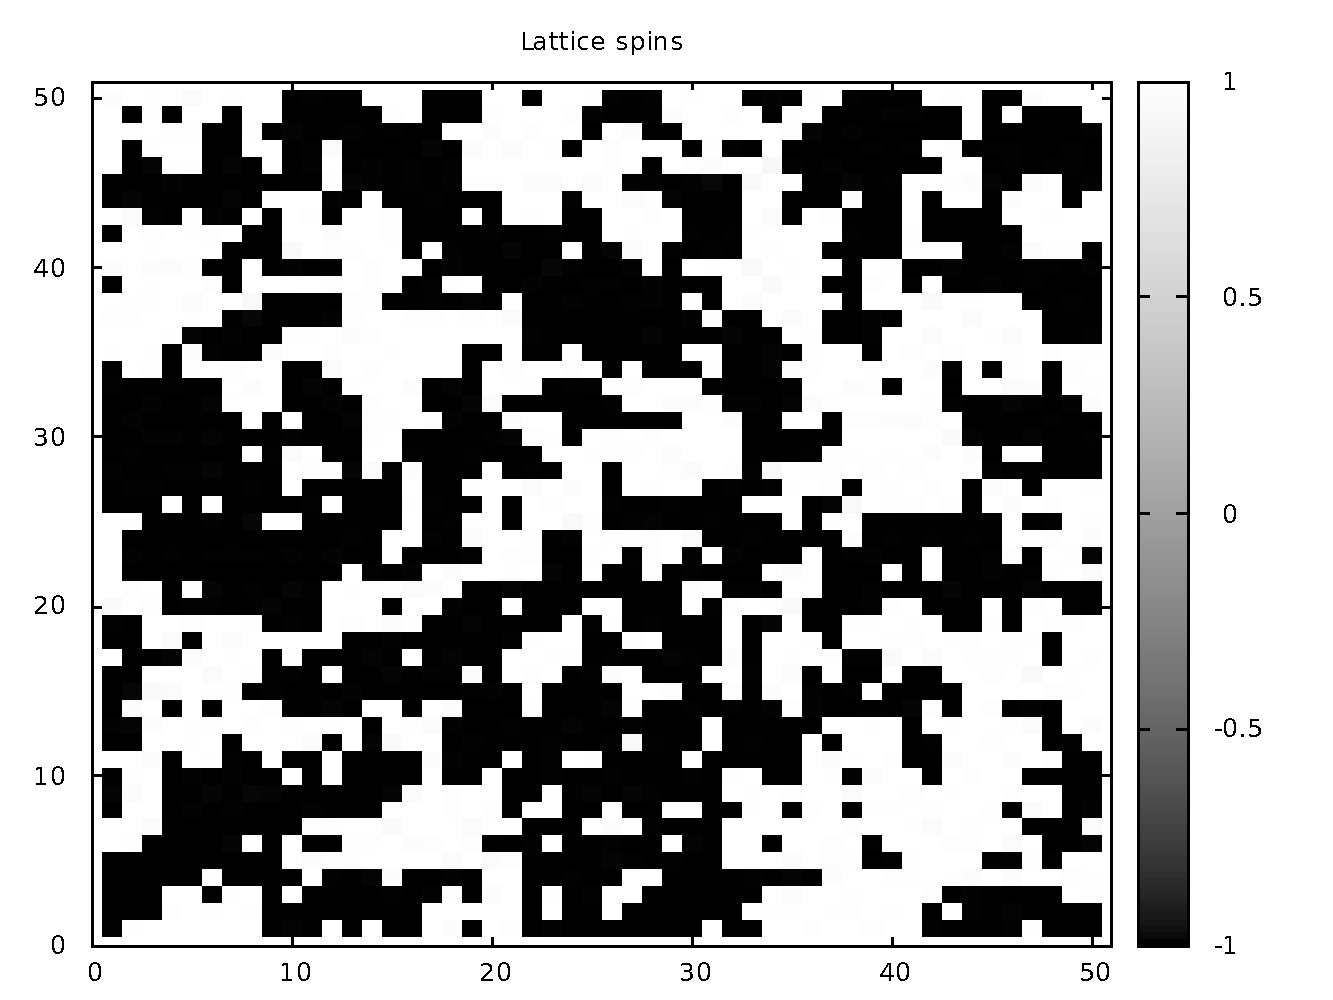
\includegraphics[width=\textwidth]{figures/spin_T_eq_3.pdf}
  \caption{$T=3$}
  \label{fig:spin_t_eq_3}
 \end{subfigure}
 
 \label{fig:spins}
 \caption{Spin at each lattice site for various temperatures.}
\end{figure}

\section{Conclusion}

\end{document}